\documentclass[a4paper]{article}
\usepackage[spanish]{babel}
\usepackage[utf8]{inputenc}
\usepackage{charter}   % tipografia
\usepackage{graphicx}
\usepackage[]{algorithm2e}
\usepackage{makeidx}
\usepackage{paralist} %itemize inline

\usepackage{multirow}

\usepackage{float}
\usepackage{amsmath, amsthm, amssymb}
\usepackage{amsfonts}
\usepackage{sectsty}
\usepackage{charter}
\usepackage{wrapfig}
\usepackage{listings}
\lstset{language=C}


\usepackage{color} % para snipets de codigo coloreados
\usepackage{fancybox}  % para el sbox de los snipets de codigo

\definecolor{litegrey}{gray}{0.94}

% \newenvironment{sidebar}{%
% 	\begin{Sbox}\begin{minipage}{.85\textwidth}}%
% 	{\end{minipage}\end{Sbox}%
% 		\begin{center}\setlength{\fboxsep}{6pt}%
% 		\shadowbox{\TheSbox}\end{center}}
% \newenvironment{warning}{%
% 	\begin{Sbox}\begin{minipage}{.85\textwidth}\sffamily\lite\small\RaggedRight}%
% 	{\end{minipage}\end{Sbox}%
% 		\begin{center}\setlength{\fboxsep}{6pt}%
% 		\colorbox{litegrey}{\TheSbox}\end{center}}

\newenvironment{codesnippet}{%
	\begin{Sbox}\begin{minipage}{\textwidth}\sffamily\small}%
	{\end{minipage}\end{Sbox}%
		\begin{center}%
		\vspace{-0.4cm}\colorbox{litegrey}{\TheSbox}\end{center}\vspace{0.3cm}}



\usepackage{fancyhdr}
\pagestyle{fancy}

%\renewcommand{\chaptermark}[1]{\markboth{#1}{}}
\renewcommand{\sectionmark}[1]{\markright{\thesection\ - #1}}

\fancyhf{}

\fancyhead[LO]{Sección \rightmark} % \thesection\ 
\fancyfoot[LO]{\small{Federico De Rocco, Manuel Casanova, Fernando Abelini}}
\fancyfoot[RO]{\thepage}
\renewcommand{\headrulewidth}{0.5pt}
\renewcommand{\footrulewidth}{0.5pt}
\setlength{\hoffset}{-0.8in}
\setlength{\textwidth}{16cm}
%\setlength{\hoffset}{-1.1cm}
%\setlength{\textwidth}{16cm}
\setlength{\headsep}{0.5cm}
\setlength{\textheight}{25cm}
\setlength{\voffset}{-0.7in}
\setlength{\headwidth}{\textwidth}
\setlength{\headheight}{13.1pt}

\renewcommand{\baselinestretch}{1.1}  % line spacing


\setcounter{secnumdepth}{2}
\usepackage{underscore}
\usepackage{caratula}
\usepackage{url}


% ******************************************************** %
%              TEMPLATE DE INFORME ORGA2 v0.1              %
% ******************************************************** %
% ******************************************************** %
%                                                          %
% ALGUNOS PAQUETES REQUERIDOS (EN UBUNTU):                 %
% ========================================
%                                                          %
% texlive-latex-base                                       %
% texlive-latex-recommended                                %
% texlive-fonts-recommended                                %
% texlive-latex-extra?                                     %
% texlive-lang-spanish (en ubuntu 13.10)                   %
% ******************************************************** %



\begin{document}


\thispagestyle{empty}
\materia{Organizaci\'on del Computador II}
\submateria{Segundo Cuatrimestre de 2014}
\titulo{Trabajo Pr\'actico II}
\subtitulo{subtitulo del trabajo}
\integrante{Federico De Rocco}{403/13}{fede.183@hotmail.com}
\integrante{Fernando Abelini}{544/09}{ferabelini@outlook.com}
\integrante{Manuel Casanova}{355/05}{casanova_manuel@yahoo.com}
\maketitle
\newpage


\thispagestyle{empty}
\vspace{3cm}
\tableofcontents
\newpage


%\normalsize
\newpage


\section{Introducci\'on}

	En este trabajo pr\'actico se pide realizar un conjunto de filtros para im\'agenes en dos lenguajes de programaci\'on, C y Assembler. Este \'ultimo debe hacerse considerando la paralelizaci\'on de los algoritmos para lograr que se puedan procesar dos p\'ixeles o m\'as en un solo ciclo. Para esto se deber\'an utilizar las instrucciones SSE. Tambi\'en se pide analizar la performance de los filtros comparando las versiones de C y de Assembler. En el siguiente informe se har\'an descripciones de los filtros pedidos y se dar\'a un an\'alisis de como se implementaron en los ya mencionados lenguajes. Se incluir\'a, por cada uno, una secci\'on experimentos en la cual se realizara las pruebas solicitadas en el enunciado. 
	
	
\section{Cropflip}
	
\subsection{Descripci\'on}

	Este filtro b\'asicamente consiste en tomar la imagen fuente, recortarla y girarla . Para esto el programa comprende como datos de entrada: src la matriz entrada(con la imagen original), dst la matriz destino, cols que contiene la cantidad de columnas, filas la cantidad de filas, $src-row-size$ que tiene el n\'umero de columnas que se debe desplazar de un elemento de la matriz para posicionarse justo en el elemento de abajo(simplemente tiene el ancho de una fila), $dst-row-size$ \'idem anterior pero de la matriz destino, tamx la cantidad de columnas en p\'ixeles a recortar, tamy la cantidad de filas en p\'ixeles a recortar, offsetx la columna, en p\'ixeles, a partir de la cual debe comenzar a recortarse, offsetxy la fila, en p\'ixeles, a partir de la cual debe comenzar a recortarse. Lo siguiente es la explicaci\'on de c\'odigo en c:
\ \\
\begin{algorithm}[H]
\ \\
$src-matriz=Matriz(src,src-row-size)$

$dst-matriz=Matriz(dst,dst-row-size)$

 \For{$i=0 ... tamy-1$}{
  \For{$j=0 ... tamx-1$}{
   $dst-matriz{i,4*j}=src-matriz[tamy+offsety-i-1][4*(offsetx+j)]$\;
   $dst-matriz{i,(4*j)+1}=src-matriz[tamy+offsety-i-1][4*(offsetx+j)+1]$\;
   $dst-matriz{i,(4*j)+2}=src-matriz[tamy+offsety-i-1][4*(offsetx+j)+2]$\;
  }
 }
\caption{Algoritmo de Cropflip en lenguaje C}
\end{algorithm}	
\ \\
	Como explicaci\'on a este seudoc\'odigo hay que agregar unos cuantos detalles. El i y el j hacen menci\'on al desplazamiento en la matriz en pixeles. Esta es la raz\'on por la cual aparece el 4* todo el tiempo junto al \'indice j. Ya que a la hora de modificar algo tenemos que hacerlo mediante los datos de los p\'ixeles los cuales son r, g, b y a. En las columnas avanzamos de a 4 para poder siempre estar posicionados en el principio de un p\'ixel. Tambi\'en al principio se pasa src y dst, que originalmente son un vector, a matrices para facilitar la explicaci\'on
	La verci\'on en assembler de este algoritmo es la siguiente:	
\ \\
\begin{algorithm}[H]
\ \\
 \For{$i=0 ... tamy-1$}{
  \For{$j=0 ... tamx-1$}{
  	$Pixel1=src[src-row-size*(tamy+offsety-i-1)+4*(offsetx+j)]$
  	$Pixel2=src[src-row-size*(tamy+offsety-i-1)+4*(offsetx+j)+1]$
  	$Pixel3=src[src-row-size*(tamy+offsety-i-1)+4*(offsetx+j)+2]$
  	$Pixel4=src[src-row-size*(tamy+offsety-i-1)+4*(offsetx+j)+3]$
 	$xmm0=[Pixel1|Pixel2|Pixel3|Pixel4]$
 	$dst[(i*dst-row-size)+j]=Pixel1$
 	$dst[(i*dst-row-size)+j+1]=Pixel2$
 	$dst[(i*dst-row-size)+j+2]=Pixel3$
 	$dst[(i*dst-row-size)+j+3]=Pixel4$
  }
 }
\caption{Algoritmo de Cropflip en lenguaje ensamblador}
\end{algorithm}	
\ \\

	Como ya no se nos facilita tanto tomar el vector con la imagen y verlo como una matriz lo que hacemos es crearnos un i y j e ir recorriendo la matriz con ellos como si fueran \'indices y hacer las ecuaciones adecuadas utiliz\'andolos. Como se trata de vectores, y m\'as concretamente posiciones de memoria de registros, estamos obligados a pensar en una forma de referirnos a una posici\'on de una estructura tipo matriz pero siendo el elemento real un simple vector de pixeles.  Cuando hacemos esta cuenta:$src-row-size*(tamy+offsety-i-1)+4*(offsetx+j)$ podemos denotar que el \'indice de fila esta multiplicado por $src-row-size$, que es el tamaño de una fila en la matriz origen, y se le suma $4*(offsetx+j)$ que es el \'indice columna. Si pensamos nos podemos das cuenta que cuando la fila sea cero esto no afectara y sencillamente recorrer\'a la primera fila de columna a columna. Cuando sea distinto a cero le sumara a la posici\'on de la columna el valor que lo ubicara en el principio de la fila que denota el \'indice correspondiente a esta. Adem\'as como se pide paralelizar en assembler, se puede ver que en el algoritmo se pasan 4 p\'ixeles de una al registro xmm0 para despu\'es escribirlo de una sola pasada en memoria. Con esto se logra en un ciclo hacer 4 veces la operaci\'on que en el de c solo se realizaba una vez. Como observaci\'on, el i avanza de a uno pero el j avanza de a 4 por las pretensiones de paralelizaci\'on expuestas anteriormente.
	El resultado de aplicar cropflip, tanto en su verci\'on C como en la de assembler, es la siguiente:
\ \\


\subsection{Experimentos}
\subsection{Experimento 1.1}

a) Las siguientes son las secciones, que no son el programa, y para que creemos que funciona cada una: 
secciones .debug*: Es informaci\'on para que utilicen los debuggers. Funciones que necesitan los debuggers para realizar ''debugueo simb\'olico''. 

sección .comment: Secci\'on donde se encuentra la informaci\'on de control de versi\'on.

sección eh_frame: Esta secci\'on contiene informaci\'on necesaria para desentrañar el frame durante el manejo de excepciones
	
b) Pone todos los par\'ametros en la pila. Coloca en la pila las variables locales y cada vez que las necesita modificar, las modifica en la porci\'on de memoria.

c) Claramente no es necesario poner tantas cosas a la pila, de esa manera se evitan acceso a memoria innecesarios. Las comparaciones de los \'indices de los ''for'', se hacen en una secci\'on apartada de c\'odigo, y cada vez que se desea ver si un ciclo debe seguir o terminar se realizan 2 saltos. En cada iteraci\'on se calcula la posici\'on de memoria a ser copiada, eso se podr\'ia evitar usando \'indices m\'oviles dentro del c\'odigo.
	
\subsection{Experimento 1.2}

a) La primera optimizaci\'on que se observa es que no tira los par\'ametros a la pila y eso le ahorra accesos a memoria al principio, mejor velocidad. Tambi\'en genera menos cantidad de c\'odigo para la funci\'on. El orden del c\'odigo es mejor(no hace dos saltos por cada ciclo).  \\
\newpage
b)\begin{center}
  \begin{tabular}{| c | c |}
    \hline
    option & optimization level\\ 
    \hline \hline
    -O0 & optimizaci\'on para el tiempo de compilaci\'on(por defecto) \\
    \hline
    -O  & optimizaci\'on para tamaño de c\'odigo y tiempo de ejecuci\'on \\
    \hline
    -O2 & optimizaci\'on para el tiempo de compilaci\'on (mejor que el anterior) \\
    \hline
    -O3 & optimizaci\'on para el tiempo de compilaci\'on (mejor que el anterior) \\
    \hline
    -Os & optimizaci\'on para el tamaño de c\'odigo \\
    \hline
    -Ofast & O3 con c\'alculos matem\'atico precisos m\'as r\'apidos \\
    \hline
  \end{tabular}
\end{center}

c) \textbf{-pipe:} Hace que el proceso de compilaci\'on sea m\'as r\'apido. Indica al compilador que use tuber\'ias en lugar de archivos temporales durante los diferentes estados de compilaci\'on, lo cual utiliza m\'as memoria.
\\ \
\textbf{-msse, -msse2, -msse3, -mmmx, -m3dnow:} Estas opciones activa instrucciones SSE, SSE2, SSE3, MMX y 3DNow para arquitecturas x86-64. 
 
\subsection{Experimento 1.3}

a) Tiempo de 10 cropflips (medidos en ticks de clock): \\
\\
\indent
\begin{tabular}{ c c }
	Implementaci\'on ASM & Implementaci\'on C\\                       
  	136442 & 689230\\
	136492 & 709210\\
	137432 & 711922\\
	139064 & 716366\\
	139164 & 716742\\
	140314 & 719720\\
	144945 & 757579\\
	145538 & 882450\\
	181304 & 974696\\
	190728 & 1000265\\	  
\end{tabular}
\\\\
\indent
\begin{tabular}{| l | c | c |}
	\hline
			& Implementaci\'on ASM & Implementaci\'on C\\
			\hline
	Promedio	 &	149142,3 & 787818\\
	Desvio	 &	19809,902 & 118500,007\\
	\hline
\end{tabular}

\begin{figure}[h]
  \centering
    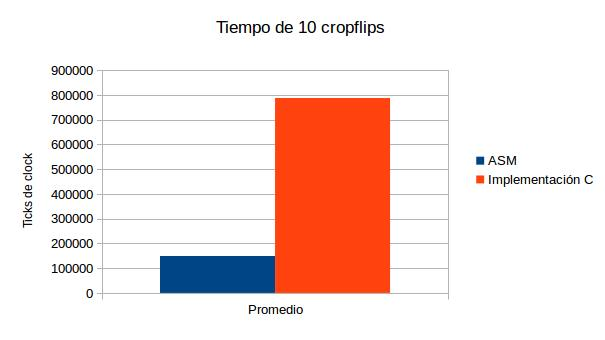
\includegraphics[width=0.7\textwidth]{1exp13a}
\end{figure}

\begin{figure}[h]
  \centering
    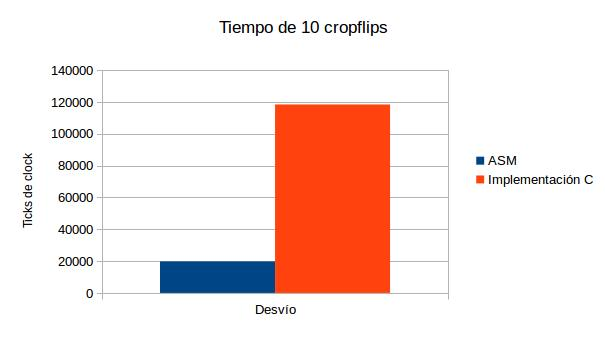
\includegraphics[width=0.7\textwidth]{1exp13b}
\end{figure}

\newpage
b) Tiempo de 10 cropflips con otros procesos dummys corriendo a la par(medidos en ticks de clock): \\
\indent

\begin{tabular}{ c c }
	Implementaci\'on asm & Implementaci\'on C\\                      
  	220151 & 1524515\\
	221788 & 1528350\\
	221867 & 1528868\\
	225978 & 1546967\\
	225984 & 1548969\\
	227241 & 1553093\\
	227273 & 1559291\\
	229922 & 1642916\\
	238021 & 1727886\\
	9021929 & 10497577\\
  
\end{tabular}

\indent
\begin{tabular}{| l | c | c |}
	\hline
			& Implementaci\'on ASM & Implementaci\'on C\\
	\hline
	Promedio	 &	1106015,4 & 2465843,2\\
	Desvio	 &	2781373,123 & 2822792,042\\
	\hline
\end{tabular}

\begin{figure}[h]
  \centering
    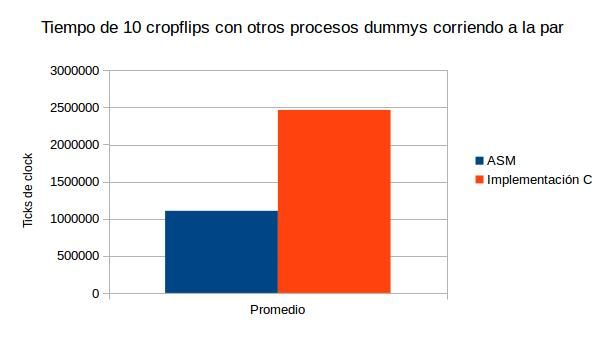
\includegraphics[width=0.7\textwidth]{1exp13c}
\end{figure}

\begin{figure}[h]
  \centering
    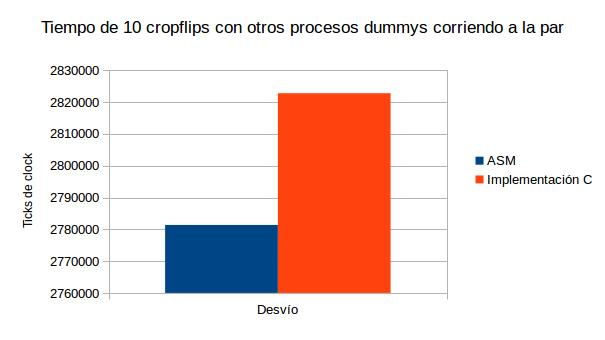
\includegraphics[width=0.7\textwidth]{1exp13d}
\end{figure}

\newpage


En los datos obtenidos se observa la existencia de números que se alejan mucho del promedio de tiempo de ejecución.
Estos números no son consecuencia de la implementación, ya que ni la maquina donde se obtuvieron los datos, ni la imagen a ser procesada fueron cambiados.
Esto se debe al funcionamiento del procesador cuando realiza un desalojo del programa y los ticks extras son el tiempo que tarda en desalojarlo y volverlo a cargar.
Los números grandes generados por el funcionamiento del procesador, hacen que las conclusiones sobre las estadísticas que saquemos sean erróneas.
De los datos obtenidos se puede concluir que:
\begin{itemize}
\item Los números grandes no son representativos de la realidad del funcionamiento de los filtros
\item Cualquier conclusión sacada de los datos que contenga a estos números (outliers)
\item los datos de las varianzas son números que aunque muestren información real, son números muy grandes para poder analizarlos, con lo que vamos a utilizar los desvíos standard.
\end{itemize}

\subsection{Experimento 1.4}


En la siguiente tabla se muestran los resultados de las versiones de ASM y C (con optimización), para comparar diferencia de performance.
Los datos se encuentran ordenados de menor a mayor. Para luego calcular promedios y desvíos quitando outliers(consideramos menor y mayor valor)
\begin{center}
\begin{tabular}{| c | c | c | c | c | }
	ASM & C	-O0 C & -O1	& C -O2	& C -O3	\\                      
	69148	& 663908	& 155642	& 164481	& 167122 \\
	75211	& 664376	& 155694	& 164501	& 167981 \\
	76054	& 664908	& 155701	& 164521	& 168318 \\
	76079	& 665380	& 155706	& 164655	& 169269 \\
	76241	& 665408	& 155771	& 165484	& 171927 \\
	76569	& 670776	& 155807	& 165644	& 172435 \\
	77480	& 674664	& 155991	& 165768	& 172949 \\
	78064	& 677812	& 156000	& 165860	& 173595 \\
	78377	& 681596	& 156437	& 166239	& 179969 \\
	103541	& 708340	& 223221	& 203650	& 192540 \\

  
\end{tabular}
\end{center}
\ \\
Calculemos ahora los promedios y desvíos est\'andar(sin outliers):\\

\begin{tabular}{| c | c | c | c | c | c | }
      \hline
	& ASM & C	-O0 C & -O1	& C -O2	& C -O3	\\   
	\hline                   
	Promedio	&	76759.375	& 670615	& 155888.375	& 165334	& 172055.375 \\
	\hline
	Desvio	&	1102.007	& 6706.207	& 253.696	& 678.080	& 3859.819 \\
	\hline

  
\end{tabular}


\begin{figure}[h]
  \centering
    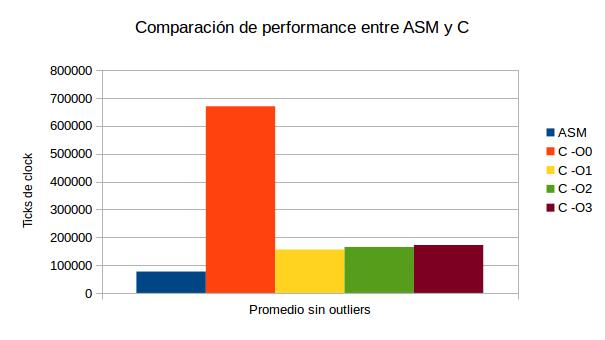
\includegraphics[width=0.7\textwidth]{1exp14a}
\end{figure}

\begin{figure}[h]
  \centering
    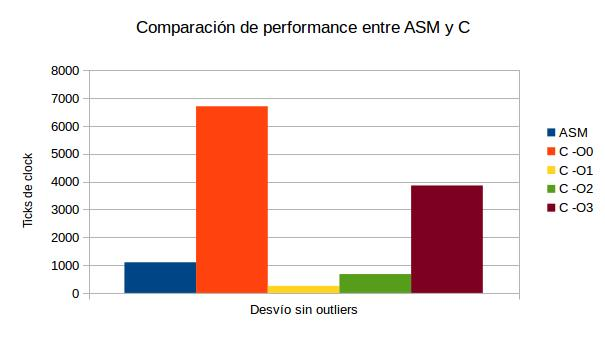
\includegraphics[width=0.7\textwidth]{1exp14b}
\end{figure}




\subsection{Experimento 1.5}


En el siguiente experimento deseamos conocer cuál es el factor limitante de la implementación en ASM. Para esto vamos a comparar los
resultados del algoritmo en ASM, contra el mismo, pero agregando operaciones aritméticas en un caso, y operaciones de acceso a memoria en otros.
La idea es verificar si lo que limita a la función son los accesos a memoria o la intensidad de cómputo.\\
En el caso de operaciones aritméticas se agregan al ciclo cierta cantidad de ADD rax, rbx.\\
En el caso de accesos a memoria se agregar 2 operaciones que leen de la pila y 2 que escriben en la pila.\\
La siguiente tabla muestra los resultados de 10 muestras:

\begin{center}
\begin{tabular}{| p{3cm} | p{3cm} | p{3cm} | p{3cm} | p{3cm} | }
	ASM	& ASM c/ accesos a memoria	& ASM c/ 4 inst aritméticas & 	ASM c/ 8 inst aritméticas & 	ASM c/ 16 inst aritméticas \\
	69148	& 61281	 & 49963	& 68062	&   105315    \\
	75211	& 62412	 & 50006	& 68325	&   105355    \\
	76054	& 63893	 & 50045	& 68869	&   109601    \\
	76079	& 64306	 & 50143	& 68894	&   110420    \\
	76241	& 64945	 & 50177	& 70784	&   111987    \\
	76569	& 65438	 & 50189	& 71283	&   113378    \\
	77480	& 66135	 & 50208	& 72280	&   115122    \\
	78064	& 67821	 & 50287	& 74418	&   117049    \\
	78377	& 74275	 & 50853	& 99932	&   121998    \\
	103541	& 172337 & 161096	& 155036 &   139228   \\


  
\end{tabular}
\end{center}
\ \\
La siguiente tabla muestra promedios y desv\'ios sin outliers:

\begin{tabular}{| p{2cm} | p{2cm} | p{2cm} | p{2cm} | p{2cm} | p{2cm} | }
      \hline
	 & ASM	& ASM c/ accesos a memoria	& ASM c/ 4 inst aritméticas	& ASM c/ 8 inst aritméticas &	ASM c/ 16 inst aritméticas	\\   
	\hline                   
	Promedio	&	76759.375	& 66153.125	& 50238.5	& 74348.125	& 113113.75 \\
	\hline
	Desvio	&	1102.007	& 3649.540	& 263.965	& 10535.389	& 5065.040
 \\
	\hline

  
\end{tabular}
\ \\

\begin{figure}[h]
  \centering
    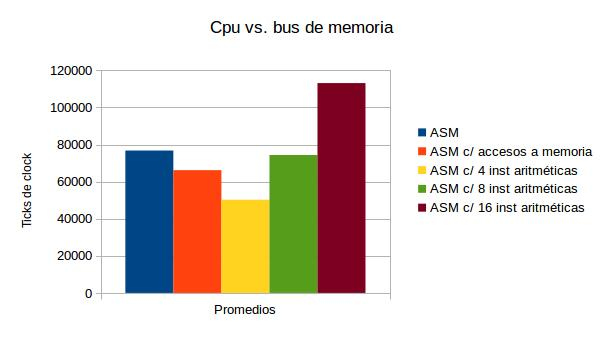
\includegraphics[width=0.7\textwidth]{1exp15a}
\end{figure}

\begin{figure}[h]
  \centering
    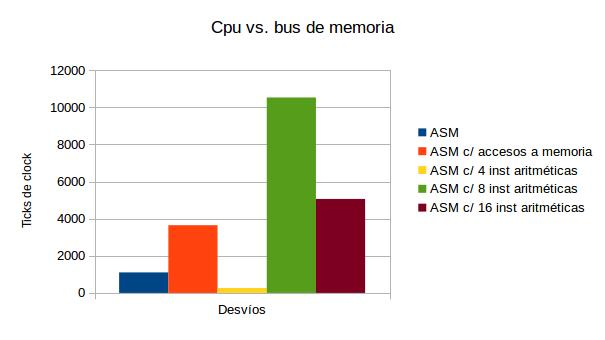
\includegraphics[width=0.7\textwidth]{1exp15b}
\end{figure}

\ \\
Como vemos en el gráfico del promedio, la implementación con accesos a memoria no significa diferencia comparada con la implementación sin modificar.
En cambio podemos ver que al agregar 16 instrucciones aritméticas los tiempos de ejecución suben considerablemente.\\
Con lo cual podemos concluir que el limitante es la intensidad de cómputo.


\section{Sierpinski}
\subsection{Descripci\'on}
El filtro de Sierpinski consiste en tomar la imagen fuente y aplicarle y aplicarle un efecto fract\'alico encima, simulando los tri\'angulos de Sierpinki pero con cuadrados. Para esto, se recorre toda la matriz de p\'ixeles, se toma la posici\'on actual y se genera un coeficiente que se multiplica por cada color en ese lugar. 
El siguiente es el algoritmo en C que implementamos para este ciclo:
\ \\
\begin{algorithm}[H]
\ \\
$src-matriz=Matriz(src,src-row-size)$

$dst-matriz=Matriz(dst,dst-row-size)$

\For{$i=0 ... tamy-1$}{
 	\For{$j=0 ... tamx-1$}{
  
		$dst-matriz{i,4*j}=src-matriz[i][(4*j)]*coef(i,j)$
   
		$dst-matriz{i,(4*j)+1}=src-matriz[i][(4*j)+1]*coef(i,j)$
   
		$dst-matriz{i,(4*j)+2}=src-matriz[i][(4*j)+2]*coef(i,j)$
   
	}
}
\caption{Algoritmo de Sierpinki en lenguaje C}
\end{algorithm}	
\ \\
Este es el algoritmo para calcular el coeficiente en C:\\
\ \\
\begin{algorithm}[H]
$ coef(i,j)=(1/255.0)*((255.0*i/CantFilas)\oplus(255.0*j/CantColumnas)) $

\end{algorithm}
 
Esto, por otro lado, es el que usamos en assembler considerando que tenemos que garantizar una cierta paralelizaci\'on de los datos:
\ \\
\begin{algorithm}[H]
\ \\
\For{$i=0 ... tamy-1$}{
  \For{$j=0 ... tamx-1$}{
  	$xmm1=[Pixel4|Pixel3|Pixel2|Pixel1]$\\
  	$Unpack de Byte a Word$\\
  	$xmm1=[Pixel2|Pixel1]$\\
  	$xmm2=[Pixel4|Pixel3]$\\
  	$Unpack de Word a DWord;$\\
  	$xmm3=[Pixel2]$\\
  	$xmm1=[Pixel1]$\\
  	$xmm2=[Pixel3]$\\
  	$xmm4=[Pixel4];$\\
  	\ \\
  	$Coef=CalcularCoeficientes$\\
  	$xmm0=|coeficiente4|coeficiente3|coficiente2|coeficiente1|$\\
  	$broadcast de los coeficientes en 4 registros para multiplicar a cada pixel$\\
  	\ \\
  	$xmm15=|coeficiente1|coeficiente1|coficiente1|coeficiente1|$
  	$xmm14=|coeficiente2|coeficiente2|coficiente2|coeficiente2|$
  	$xmm13=|coeficiente3|coeficiente3|coficiente3|coeficiente3|$
  	$xmm12=|coeficiente4|coeficiente4|coficiente4|coeficiente4|$
  	\ \\
  	$ConvertimosAPresicionSimple(xmm1)$\\
  	$ConvertimosAPresicionSimple(xmm2)$\\
  	$ConvertimosAPresicionSimple(xmm3)$\\
  	$ConvertimosAPresicionSimple(xmm4)$\\
  	\ \\
  	$xmm1=xmm1*xmm15$\\
  	$xmm2=xmm2*xmm14$\\
  	$xmm3=xmm3*xmm13$\\
  	$xmm4=xmm4*xmm12$\\
  	\ \\
  	$ConvertimosAEnteros(xmm1)$\\
  	$ConvertimosAEnteros(xmm2)$\\
  	$ConvertimosAEnteros(xmm3)$\\
  	$ConvertimosAEnteros(xmm4)$\\
  	\ \\
  	$Pack DWord a Word$\\
  	$xmm2=[Pixel4, Pixel3]$\\
  	$xmm1=[Pixel2, Pixel1]$\\
  	$Pack Word a Byte$\\
  	$xmm1=[Pixel4|Pixel3|Pixel2|Pixel1]$\\
  	$return\ xmm1$
  }
}
\caption{Algoritmo de Sierpinki en lenguaje ensamblador}
\end{algorithm}	
\ \\
\newpage
\subsection{Experimentos}
\subsection{Experimento 2.1}

\textbf{Secuencial vs Vectorial} \\
Se realizó la siguiente medición para comparar la performance de las versiones de C y ASM. Para esto se midió el tiempo de el algoritmo
sierpinski en ASM y en C compilado con las diferentes opciones de optimización(-O0 -O1 -O2 -O3 ) \\

Se obtiene la siguiente tabla de resultados: \\

\begin{center}
  \begin{tabular}{| c | c | c | c | c |}
    \hline
    ASM & C -O0 & C -O1 & C -O2 & C -O3\\ 
    \hline\hline
	1979149 & 23950764	& 24978220	& 23956842	& 23945653 \\
	\hline                                                 
	1979591 & 23950966	& 25046817	& 23984700	& 23961380 \\
	\hline                                                 
	1983075 & 24002597	& 25246046	& 24016093	& 23971489 \\
	\hline                                                 
	2046425 & 24003697	& 25316344	& 24039011	& 24006034 \\
	\hline                                                 
	2311542 & 24045930	& 25349957	& 24069702	& 24019744 \\
	\hline                                                 
	2493975 & 24056933	& 25373885	& 24077508	& 24022409 \\
	\hline                                                 
	2605145 & 24203169	& 25411694	& 24105201	& 24180257 \\
	\hline                                                 
	2792657 & 24216998	& 25936224	& 24347966	& 24314764 \\
	\hline                                                 
	2838663 & 24233878	& 26082798	& 24363335	& 24446882 \\
	\hline                                                 
	2948310 & 26538594	& 26733527	& 26753905	& 26513368 \\
	\hline
  \end{tabular}
\end{center}
\ \\

\begin{figure}[h]
  \centering
    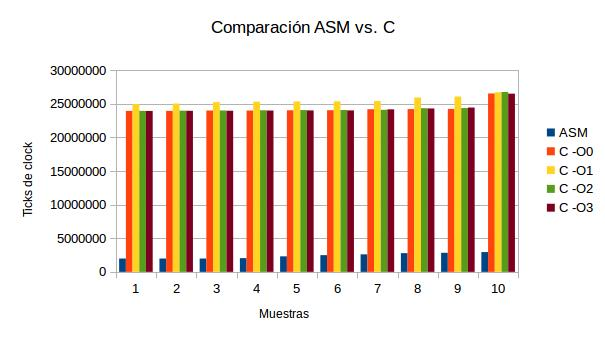
\includegraphics[width=0.7\textwidth]{1exp21}
\end{figure}
\ \\
Se puede ver que los tiempos de ASM con respecto a C con cualquier nivel de optimización son superiores. Calculemos Promedios y desv\'ios est\'andar
de los datos, descartando outliers(el menor y mayor valor)\\ 

\begin{center}
  \begin{tabular}{| c | c | c | c | c | c |}
    \hline
      & ASM & C -O0 & C -O1 & C -O2 & C -O3 \\
      \hline\hline
      Promedio	& 2381384.125	& 24089271 & 25470470.625 & 24125439.5 & 24115369.875\\
      \hline
      Desvio estandard & 354190 & 111538 & 353104 & 146950 & 180484 \\
      \hline

  \end{tabular}
\end{center}

\begin{figure}[h]
  \centering
    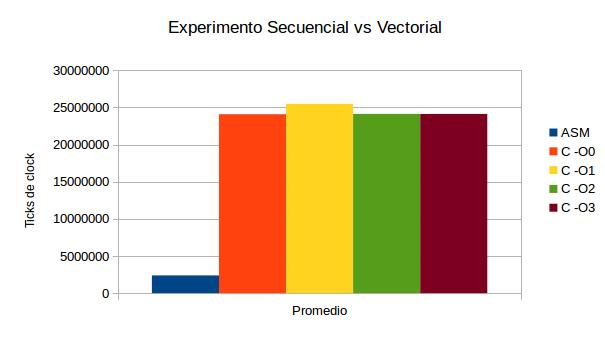
\includegraphics[width=0.7\textwidth]{1exp21promedios}
\end{figure}

\begin{figure}[h]
  \centering
    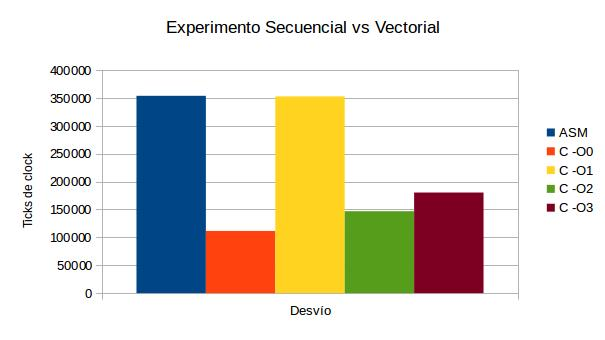
\includegraphics[width=0.7\textwidth]{1exp21desvio}
\end{figure}
\ \\
\newpage
Verifiquemos ahora la performance del filtro con procesos corriendo a la par. Para esto ejecutamos un programa por cada core lógico
que cicla infinitamente sumando 1 a una variable.

\ \\

\begin{center}
  \begin{tabular}{| c | c | c | c | c |}
    \hline
    ASM & C -O0 & C -O1 & C -O2 & C -O3\\ 
    \hline\hline
  3670735	& 41244828	& 30835911	& 30596371	& 30743988 \\
  \hline
  3672513	& 44918524	& 30861208	& 30738494	& 30755299 \\
  \hline
  3673100	& 45245188	& 40615205	& 30757275	& 30756271 \\
  \hline
  3677214	& 51538693	& 41101907	& 30764515	& 30759578 \\
  \hline
  3684686	& 51626548	& 41226423	& 30772374	& 39228198 \\
  \hline
  3685366	& 51634223	& 51560508	& 30772609	& 42790292 \\
  \hline
  3700843	& 51645082	& 52257507	& 30801802	& 51483986 \\
  \hline
  3713232	& 51652554	& 52499858	& 30818767	& 51504201 \\
  \hline
  3736790	& 51704539	& 54523487	& 32069388	& 51533906 \\
  \hline 
  4624072	& 52573857	& 61887910	& 72290370	& 63653873 \\
  \hline
  \end{tabular}
\end{center}

\begin{figure}[h]
  \centering
    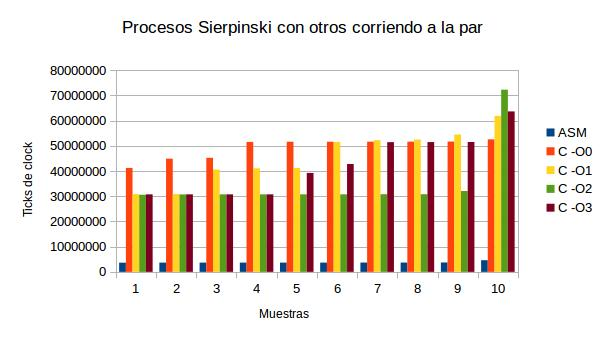
\includegraphics[width=0.7\textwidth]{2exp21}
\end{figure}
\ \\
\newpage
\begin{center}
  \begin{tabular}{| c | c | c | c | c | c |}
    \hline
      & ASM & C -O0 & C -O1 & C -O2 & C -O3 \\
      \hline\hline
      Promedio	& 3692968 & 49995668.875 & 45580762.875 & 30936903 & 41101466.375\\
      \hline
      Desvio est\'andar & 22617 & 3034470 & 8353997 & 458279 & 9652768 \\
      \hline

  \end{tabular}
\end{center}

\begin{figure}[h]
  \centering
    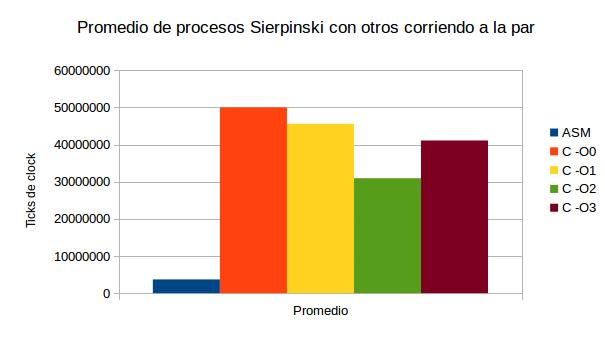
\includegraphics[width=0.7\textwidth]{2exp21promedios}
\end{figure}
\begin{figure}[h]
  \centering
    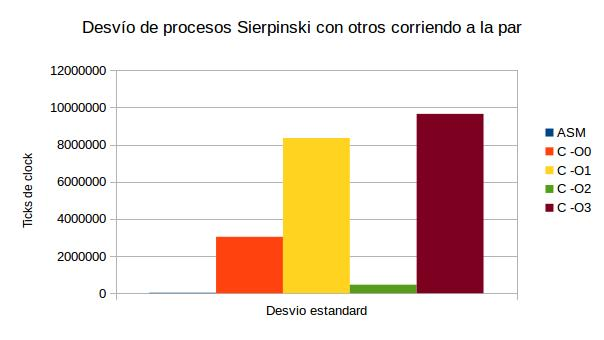
\includegraphics[width=0.7\textwidth]{2exp21desvio}
\end{figure}

\newpage
\subsection{Experimento 2.2}
\textbf{CPU vs bus de memoria}\\
Realizamos experimento para verificar que factor es el mayor limitante de la performance la versión ASM de sierpinski.
Para esto comparamos los tiempos del código original contra uno modificado, agregando instrucciones aritméticas o instrucciones
que realicen accesos a memoria.\\
Se obtienen los siguientes resultados:\\

\begin{center}
  \begin{tabular}{| c | c |}
    \hline
      ASM original & ASM agregando accesos a memoria \\
      \hline\hline
		2940985	& 2886240  \\
		\hline
		2115091	& 2228486  \\
		\hline
		2113430	& 2280717  \\
		\hline
		2450323	& 2582231  \\
		\hline
		2806890	& 2818483  \\
		\hline
		2847948	& 2617010  \\
		\hline
		2830241	& 3999342  \\
		\hline
		2116241	& 2309797  \\
		\hline
		2152194	& 2111518  \\
		\hline
		2044160	& 2104327  \\
		\hline


  \end{tabular}
\end{center}
\ \\


\begin{center}
  \begin{tabular}{| p{3cm} | p{3cm} | p{3cm} | p{3cm} |}
    \hline
       ASM original & Asm c/ 4 instrucciones aritm\'eticas & Asm c/ 8 instrucciones aritm\'eticas & Asm c/ 16 instrucciones aritm\'eticas \\
      \hline\hline
		2940985	& 3382576	& 2829676	& 2378403 \\
		\hline
		2115091	& 3219106	& 2839452	& 2448264\\
		\hline
		2113430	& 2184028	& 2840240	& 2452696\\
		\hline
		2450323	& 2195801	& 2842240	& 4327147\\
		\hline
		2806890	& 2419465	& 2855848	& 4507762\\
		\hline
		2847948	& 2932075	& 4444074	& 4841270\\
		\hline
		2830241	& 3396019	& 5630711	& 5592174\\
		\hline
		2116241	& 2831709	& 5967198	& 6113666\\
		\hline
		2152194	& 2030719	& 6050832	& 6165354\\
		\hline
		2044160	& 2268153	& 7446114	& 6189698\\
		\hline

  \end{tabular}
\end{center}

\ \\
Calculamos promedios, descartando outliers. \\

\begin{center}
  \begin{tabular}{| p{2cm} | p{2cm} | p{2cm} | p{2cm} | p{2cm} | p{2cm} |}
    \hline
      & ASM & ASM c/ accesos a memoria  &Asm c/ 4 instrucciones aritm\'eticas & Asm c/ 8 instrucciones aritm\'eticas & Asm c/ 16 instrucciones aritm\'eticas \\
      \hline\hline
      Promedios sin outliers & 2429044 & 2618448 & 2651115 & 4183824 & 4556041 \\
      \hline

  \end{tabular}
\end{center}


\begin{figure}[h]
  \centering
    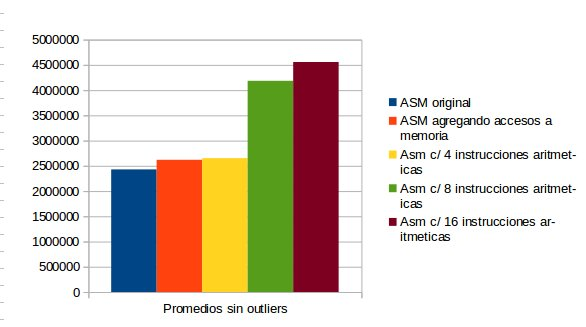
\includegraphics[width=0.7\textwidth]{exp34}
\end{figure}

\ \\
De la misma forma que en el filtro Cropflip. Podemos ver por el gráfico anterior que el limitante es la intensidad de cómputo. Ya que 
el tiempo de ejecución aumenta a medida que se agregar operaciones aritméticas. En cambio con accesos a memoria no hay tanta diferencia.


\section{Bandas}
\subsection{Descripci\'on}

	El filtro bandas sirve para, en t\'erminos simples, pasar una imagen de color a una en varios tonos de gris(blanco y negro). La forma de realizar esto es revisar p\'ixel a p\'ixel de la imagen y analizar el valor de la suma de los componentes R, G y B:
\ \\	
$b_{i,j}=src.r_{i,j}+src.g_{i,j}+src.b_{i,j}$
\ \\
A los pixeles de la imagen destino se les da valores basado en la siguiente ecuaci\'on. 
\ \\
\[ dsp(i,j) <r,g,b> = \left\{ 
  \begin{array}{l l}
    <0,0,0> & \quad \text{$b<96$}\\
    <64,64,64>  & \quad \text{$96<=b<288$}\\
    <128,128,128>  & \quad \text{$288<=b<480$}\\
    <192,192,192>  & \quad \text{$480<=b<672$}\\
    <255,255,255>  & \quad \text{si no}
  \end{array} \right.\]





El siguiente es el seudoc\'odigo de bandas en C:
\ \\
\begin{algorithm}[H]
\ \\
$src-matriz=Matriz(src,src-row-size)$

$dst-matriz=Matriz(dst,dst-row-size)$

 \For{$i=0 ... tamy-1$}{
  \For{$j=0 ... tamx-1$}{
   $suma = src-matriz_{i,j}.r+src-matriz_{i,j}.g+src-matriz_{i,j}.b$\;
   \If{$suma<96$}{
      $dst-matriz_{i,j}.r=0$\;
      $dst-matriz_{i,j}.g=0$\;
      $dst-matriz_{i,j}.b=0$\;
   }
   \If{$96<=suma<288$}{
      $dst-matriz_{i,j}.r=64$\;
      $dst-matriz_{i,j}.g=64$\;
      $dst-matriz_{i,j}.b=64$\;
   }
   \If{$288<=suma<480$}{
      $dst-matriz_{i,j}.r=128$\;
      $dst-matriz_{i,j}.g=128$\;
      $dst-matriz_{i,j}.b=128$\;
   }
   \eIf{$480<=suma<672$}{
      $dst-matriz_{i,j}.r=192$\;
      $dst-matriz_{i,j}.g=192$\;
      $dst-matriz_{i,j}.b=192$\;
  }{  $dst-matriz_{i,j}.r=255$\;
      $dst-matriz_{i,j}.g=255$\;
      $dst-matriz_{i,j}.b=255$\;}
 }
 }
\caption{Algoritmo de Bandas en lenguaje C}
\end{algorithm}	
\ \\

En el caso del Asm, para poder paralelizar se toma una muestra de cuatro p\'ixeles. Despu\'es se la divide en tres registros de 128 bits para poder tener en cada uno un solo color. Se los suma cada cual con el correspondiente y se ve a que banda pertenece cada uno.
Este seudoc\'odigo lo explica:
\ \\
\begin{algorithm}[H]
\ \\
$src-matriz=Matriz(src,src-row-size)$

$dst-matriz=Matriz(dst,dst-row-size)$

 \For{$i=0 ... tamy-1$}{
  \For{$j=0 ... tamx-1$}{
   $xmm0 = [Pixel1|Pixel12|Pixel3|Pixel4]$\;
   $xmm1 = [Pixel1.r|Pixel12.r|Pixel3.r|Pixel4.r]$\;
   $xmm2 = [Pixel1.g|Pixel12.g|Pixel3.g|Pixel4.g]$\;
   $xmm3 = [Pixel1.b|Pixel12.b|Pixel3.b|Pixel4.b]$\;
   $xmm0=[Pixel1.r+Pixel1.g+Pixel1.b|Pixel2.r+Pixel2.g+Pixel2.b|Pixel3.r+Pixel3.g+Pixel3.b|Pixel4.r+Pixel4.g+Pixel4.b]$\;
   \If{$xmm0[1,2,3,4]<96$}{
      $dst-matriz_{i,j},dst-matriz_{i,j+1},dst-matriz_{i,j+2},dst-matriz_{i,j+3}.r=0$\;
      $dst-matriz_{i,j},dst-matriz_{i,j+1},dst-matriz_{i,j+2},dst-matriz_{i,j+3}.g=0$\;
      $dst-matriz_{i,j},dst-matriz_{i,j+1},dst-matriz_{i,j+2},dst-matriz_{i,j+3}.b=0$\;
   }
   \If{$96<=xmm0[1,2,3,4]<288$}{
      $dst-matriz_{i,j},dst-matriz_{i,j+1},dst-matriz_{i,j+2},dst-matriz_{i,j+3}.r=64$\;
      $dst-matriz_{i,j},dst-matriz_{i,j+1},dst-matriz_{i,j+2},dst-matriz_{i,j+3}.g=64$\;
      $dst-matriz_{i,j},dst-matriz_{i,j+1},dst-matriz_{i,j+2},dst-matriz_{i,j+3}.b=64$\;
   }
   \If{$288<=xmm0[1,2,3,4]<480$}{
      $dst-matriz_{i,j},dst-matriz_{i,j+1},dst-matriz_{i,j+2},dst-matriz_{i,j+3}.r=128$\;
      $dst-matriz_{i,j},dst-matriz_{i,j+1},dst-matriz_{i,j+2},dst-matriz_{i,j+3}.g=128$\;
      $dst-matriz_{i,j},dst-matriz_{i,j+1},dst-matriz_{i,j+2},dst-matriz_{i,j+3}.b=128$\;
   }
   \eIf{$480<=xmm0[1,2,3,4]<672$}{
      $dst-matriz_{i,j},dst-matriz_{i,j+1},dst-matriz_{i,j+2},dst-matriz_{i,j+3}.r=192$\;
      $dst-matriz_{i,j},dst-matriz_{i,j+1},dst-matriz_{i,j+2},dst-matriz_{i,j+3}.g=192$\;
      $dst-matriz_{i,j},dst-matriz_{i,j+1},dst-matriz_{i,j+2},dst-matriz_{i,j+3}.b=192$\;
  }{  $dst-matriz_{i,j},dst-matriz_{i,j+1},dst-matriz_{i,j+2},dst-matriz_{i,j+3}.r=255$\;
      $dst-matriz_{i,j},dst-matriz_{i,j+1},dst-matriz_{i,j+2},dst-matriz_{i,j+3}.g=255$\;
      $dst-matriz_{i,j},dst-matriz_{i,j+1},dst-matriz_{i,j+2},dst-matriz_{i,j+3}.b=255$\;}
 }
 }
\caption{Algoritmo de Bandas en lenguaje ensamblador}
\end{algorithm}	
\ \\
Como aclaraci\'on al c\'odigo anterior hay que agregar que cada uno de los if lo que hace es fijarse cuales cumplen la condici\'on y solo aplica la banda a los que la cumplen. En la explicaci\'on anterior puede no quedar tan claro pero en la implementaci\'on funciona correctamente.

\subsection{Experimentos}
\subsection{Experimento 3.1}
Iniciamos el experimento evaluando la performance del c\'odigo en C utilizando el flag -O1. En este caso no cambiamos la implementaci\'on.
\ \\
Las diez mediciones de tiempo:
\ \\
\begin{center}
  \begin{tabular}{| c |}
    \hline
    Com\'un\\ 
    \hline\hline
    12797809\\
    \hline
    11358186\\
    \hline
    11456151\\
    \hline
    11293769\\
    \hline
    11472111\\
    \hline
    11471974\\
    \hline
    11450355\\
    \hline
    11362942\\
    \hline
    11477382\\
    \hline
    11391629\\
    \hline
  \end{tabular}
\end{center}
\ \\
La esperanza para estas mediciones es de 11553230,8 y su varianza de 441664,378.
\ \\
\begin{center}
  \begin{tabular}{| c |}
    \hline
    Con los procesos corriendo al mismo tiempo\\ 
    \hline\hline
    23654158\\
    \hline
    16879559\\
    \hline
    27527850\\
    \hline
    34991082\\
    \hline
    25223929\\
    \hline
    20965508\\
    \hline
    31951311\\
    \hline
    22588902\\
    \hline
    16661662\\
    \hline
    15221451\\

    \hline
  \end{tabular}
\end{center}
\ \\
La esperanza para estas mediciones es de 23566541,2 y su varianza de 6574579,37641277.
\ \\
\begin{center}
  \begin{tabular}{| c |}
    \hline
    Sin los outliers\\ 
    \hline\hline
    11456151\\ 
    \hline
    11472111\\ 
    \hline
    11471974\\ 
    \hline
    11450355\\ 
    \hline
    11362942\\ 
    \hline
    11391629\\ 
    \hline
  \end{tabular}
\end{center}
\ \\
La esperanza para estas mediciones es de 11434193,666 y su varianza de 45819,082.


\begin{figure}[h]
  \centering
    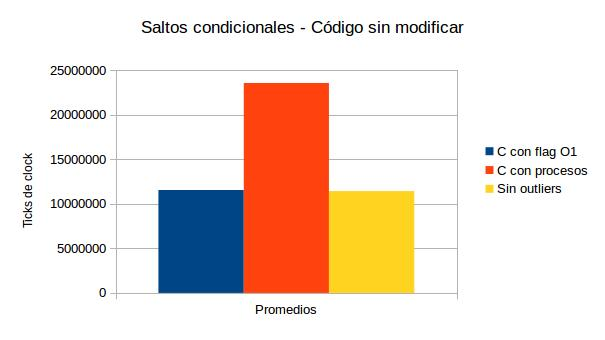
\includegraphics[width=0.7\textwidth]{1exp31a}
\end{figure}

\begin{figure}[h]
  \centering
    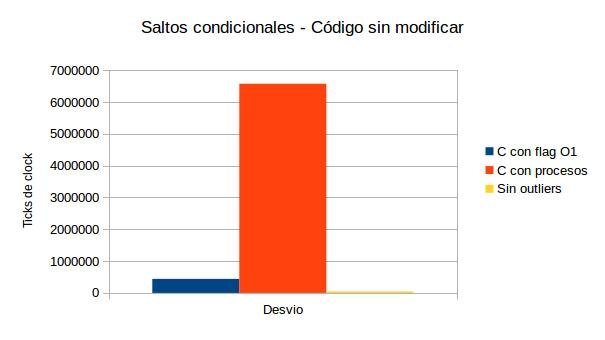
\includegraphics[width=0.7\textwidth]{1exp31b}
\end{figure}


\ \\
Ahora veamos que pasa en el caso de que modifiquemos el c\'odigo y solo dejemos una banda.
\ \\
\begin{center}
  \begin{tabular}{| c |}
    \hline
    Com\'un con c\'odigo cambiado\\ 
    \hline\hline
    12436809\\
    \hline
    11426194\\
    \hline
    11446638\\
    \hline
    11500629\\
    \hline
    11287762\\
    \hline
    11280833\\
    \hline
    11780128\\
    \hline
    11297695\\
    \hline
    11351046\\
    \hline
    11389654\\
    \hline
  \end{tabular}
\end{center}
\ \\
La esperanza para estas mediciones es de 11519738,8 y su varianza de 354158,127.
\begin{center}
  \begin{tabular}{| c |}
    \hline
    Con los procesos corriendo al mismo tiempo\\ 
    \hline\hline
    20866272\\
    \hline
    11749017\\
    \hline
    11300268\\
    \hline
    11354311\\
    \hline
    11275667\\
    \hline
    11349775\\
    \hline
    11321804\\
    \hline
    13787571\\
    \hline
    11277630\\
    \hline
    30533381\\
    \hline
  \end{tabular}
\end{center}
\ \\
La esperanza para estas mediciones es de 14481569,6 y su varianza de 6382347,830.
\ \\
\ \\
\begin{center}
  \begin{tabular}{| c |}
    \hline
    Com\'un con c\'odigo cambiado\\ 
    \hline\hline
    11426194\\
    \hline
    11446638\\
    \hline
    11500629\\
    \hline
    11297695\\
    \hline
    11351046\\
    \hline
    11389654\\
    \hline
  \end{tabular}
\end{center}
\ \\
La esperanza para estas mediciones es de 11401976 y su varianza de 72019,224.
\ \\


\begin{figure}[h]
  \centering
    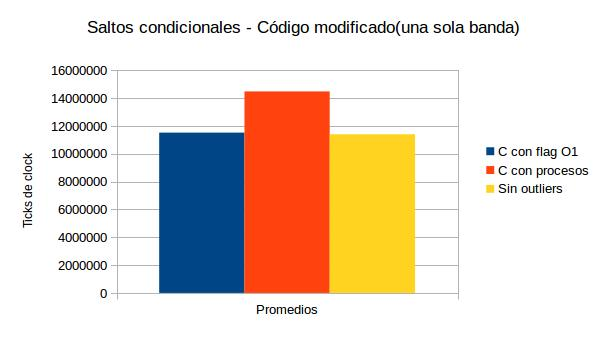
\includegraphics[width=0.7\textwidth]{1exp31c}
\end{figure}


\begin{figure}[h]
  \centering
    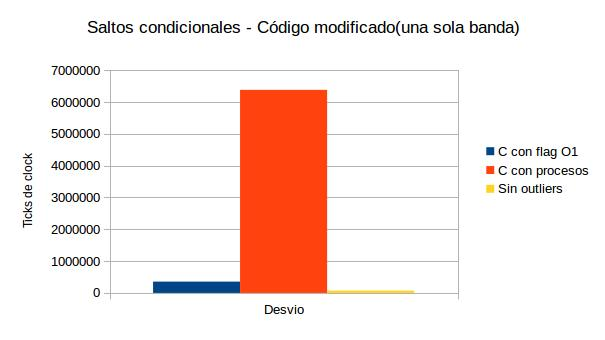
\includegraphics[width=0.7\textwidth]{1exp31d}
\end{figure}


Como concluci\'on podemos observar que hay diferencia en todos los promedios. Esto muestra que al haber menos saltos condicionales mejor performance se puede obtener.
\subsection{Experimento 3.2}
Se toma, al igual que en Sierpinski, una muestra de 10 tiempos como se muestra en el siguiente cuadro.
\begin{center}
  \begin{tabular}{| c | c | c | c | c | c | c |}
    \hline
    ASM & C Com\'un &C -O0 & C -O1 & C -O2 & C -O3\\ 
    \hline\hline
    3505918 &22135543 & 12641517 & 6063488 &4942045 &4954026\\
    \hline
    2589290 &20564901 & 11374010 & 4370152 &3735952 &3706931\\
    \hline
    2542470 &14731584 & 11354143 &4356261 &3675945 &3761121\\
    \hline
    2534196 &12061801 & 11537515 &4376631 &3712537& 3716506\\
    \hline
    2532852 &11766793 & 11393466 & 4304202 &3728077 &3734503\\
    \hline
    2532789 &14631057 & 11318969 &4307278 &3653412 &3823449\\
    \hline
    2557916 &15051960 & 11323085  &4329139 &3650608 &3754663\\
    \hline
    2533167 &18488820 & 11380404 & 4302995 &3678528 &3751923\\
    \hline
    2533650 &28220955 & 11461653 & 4319343 &3768387 &3796926\\
    \hline
    2534175 &15310701 & 11364076 & 4301430 &3690456 &3757289\\
    \hline
  \end{tabular}
\end{center}

\begin{center}
  \begin{tabular}{| c | c | c | c | c | c | c |}
    \hline
      & ASM & C Com\'un& C -O0 & C -O1 & C -O2 & C -O3 \\
      \hline\hline
      Promedio	& 2639642,3 &17296411,5 & 11514883,8  &4503091,9 &3823594,7 &3875733,7\\
      \hline
      Desv\'io est\'andar & 304909,096 &5115429,788  &401257,823  &549008,248 &394767,849  &380439,069\\
      \hline
  \end{tabular}
\end{center}


\begin{figure}[h]
  \centering
    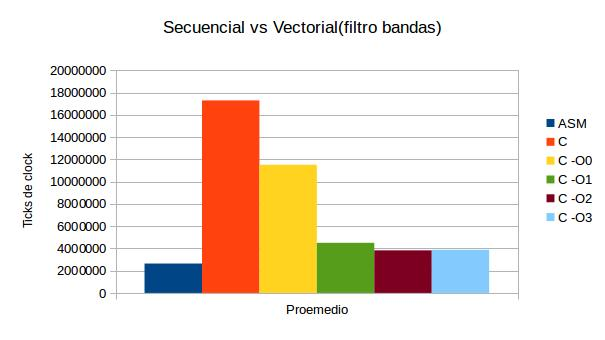
\includegraphics[width=0.7\textwidth]{1exp32a}
\end{figure}


\begin{figure}[h]
  \centering
    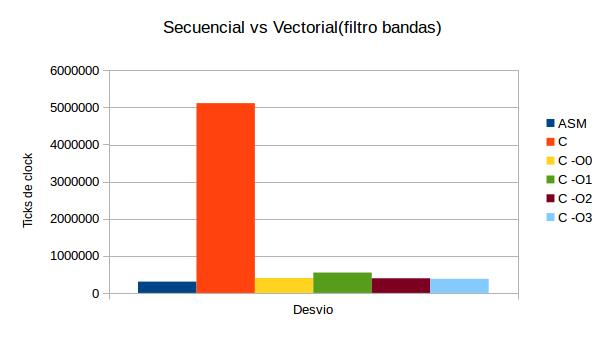
\includegraphics[width=0.7\textwidth]{1exp32b}
\end{figure}


\ \\
Con los procesos de los cores l\'ogicos:
\ \\
\begin{center}
  \begin{tabular}{| c | c | c | c | c | c | c |}
    \hline
    ASM & C Com\'un &C -O0 & C -O1 & C -O2 & C -O3\\ 
    \hline\hline
    3520388 &40116269  &37608428  &28102158  &8617277 &5064644\\
    \hline
    2593217 &22731334  &22614501 &4672825& 3659492 &3700715\\
    \hline
    5670735 &13091673  &24022404 &16448796  &3740572 &3698320\\
    \hline
    2658001 &11822485  &11310001 &13676554  &3657665 &3716433\\
    \hline
    2575713 &26133355  &22537746 &9039156 &15063752 & 3703833\\
    \hline
    2538091 &11627679  &24434225 &19962600  &5914944 &3704757\\
    \hline
    9665964 &17933191  &20460184 &4367391 &6998639& 3698814\\
    \hline
    2639889 &20779059  &22565466 &4385083 &23254434 & 4195769\\
    \hline
    2672597 &12737771  &11301497 &4397085 &3698772 &3899291\\
    \hline
    2933228 &12931149  &29606566 &4304727 &7139958 &3749571\\
    \hline

    \hline
  \end{tabular}
\end{center}

\ \\
\begin{center}
  \begin{tabular}{| c | c | c | c | c | c | c |}
    \hline
      & ASM & C Com\'un& C -O0 & C -O1 & C -O2 & C -O3 \\
      \hline\hline
      Promedio	& 3746782,3  &18990396,5 & 22646101,8  &10935637,5 & 8174550,5 &3923080,5\\
      \hline
      Desv\'io est\'andar & 2289566,028& 9017447,683 & 7741773,966 & 8364446,914 &6351725,293&  429928,854\\
      \hline
  \end{tabular}
\end{center}


\begin{figure}[h]
  \centering
    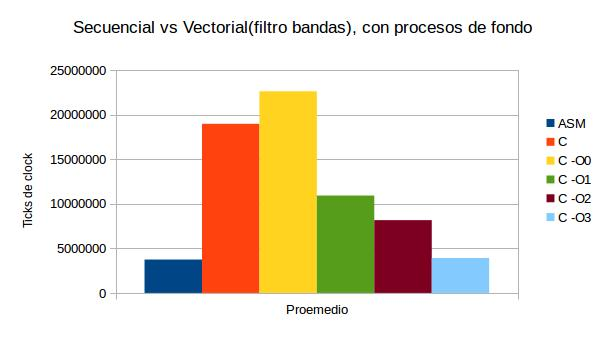
\includegraphics[width=0.7\textwidth]{1exp32c}
\end{figure}

\begin{figure}[h]
  \centering
    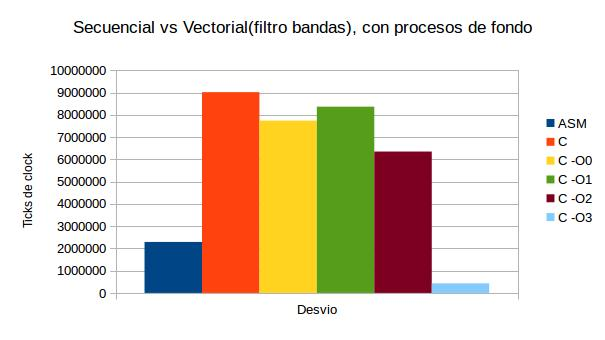
\includegraphics[width=0.7\textwidth]{1exp32d}
\end{figure}



\ \\
Sin los outliers:
\ \\
\begin{center}
  \begin{tabular}{| c | c | c | c | c | c | c |}
    \hline
    ASM & C Com\'un &C -O0 & C -O1 & C -O2 & C -O3\\ 
    \hline\hline
    2542470 &20564901  &11374010 &4370152 &3675945 &3761121\\
    \hline
    2534196 &14731584  &11354143 &4356261 &3712537 &3734503\\
    \hline
    2557916 &15310701  &11393466 &4319343 &3728077 &3754663\\
    \hline
    2533167 &14631057  &11380404 &4304202 &3678528 &3751923\\
    \hline
    2533650 &15051960  &11461653 &4307278 &3768387 &3796926\\
    \hline
    2534175 &18488820  &11364076 &4329139 &3690456 &3757289\\
    \hline
  \end{tabular}
\end{center}
\ \\

\begin{center}
  \begin{tabular}{| c | c | c | c | c | c | c |}
    \hline
      & ASM & C Com\'un& C -O0 & C -O1 & C -O2 & C -O3 \\
      \hline\hline
      Promedio	& 2539262,3336 &16463170,5 & 11387958,666 & 4331062,5& 63708988,333 &3759404,166\\
      \hline
      Desv\'io est\'andar & 9782,110&  2473951,563&  38540,121&  26799,958& 35407,098&  20561,245\\
      \hline
  \end{tabular}
\end{center}
\ \\

\begin{figure}[h]
  \centering
    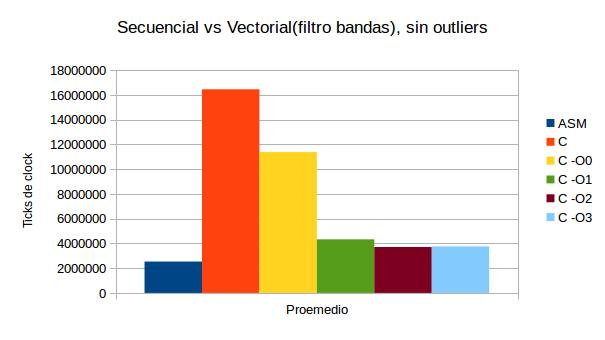
\includegraphics[width=0.7\textwidth]{1exp32e}
\end{figure}

\begin{figure}[h]
  \centering
    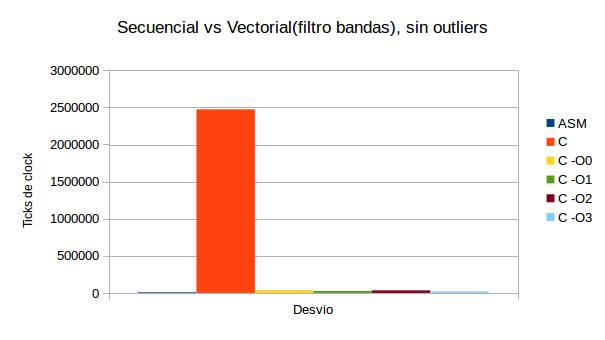
\includegraphics[width=0.7\textwidth]{1exp32f}
\end{figure}


Como podemos ver en cada una de las mediciones, tenemos que el c\'odigo en ensamblador presenta siempre mejor desempeño respecto al de C con cualquiera de los flags. En cuanto al de C tenemos que la mejora de los flags parece ser ascendente. 
\section{Motion Blur}
\subsection{Descripci\'on}
Este filtro toma una imagen de entrada y le aplica un efecto de desenfoque de movimiento. Para lograr esto se tiene que aplicar la siguiente funci\'on de cada p\'ixel:
\ \\
$dst_{i,j}=0,2*src_{i-2,j-2}+0,2*src_{i-1,j-1}+0,2*src_{i,j}+0,2*src_{i+1,j+1}+0,2*src_{i+2,j+2}$
\ \\
La funci\'on toma partes del valor de sus vecinos. Los bordes se pintan de negro por no ser posible calcular la anterior ecuaci\'on. 

$dst_{i,j}=0 si i<2 \vee j<2 \vee i+2>=tamy \vee j+2>=tamx$

El siguiente es el seudoc\'odigo asociado al filtro motion blur en la implementaci\'on en C:

\ \\
\begin{algorithm}[H]

$src-matriz=Matriz(src,src-row-size)$

$dst-matriz=Matriz(dst,dst-row-size)$


\For{$i=0...filas-1$}{
	\For{$j=0...cols-1$}{
		\eIf{$i<2\ or\ j<2\ or\ i+2>=tamy\ or\ j+2>=tamx$}{
			$dst-matriz_{i,j}=0 $\\
		}{
			$dst-matriz_{i,j}.r=0,2*src-matriz_{i-2,j-2}.r+0,2*src-matriz_{i-1,j-1}.r+0,2*src-matriz_{i,j}.r+0,2*src-matriz_{i+1,j+1}.r+0,2*src-matriz_{i+2,j+2}.r$
			$dst-matriz_{i,j}.g=0,2*src-matriz_{i-2,j-2}.g+0,2*src-matriz_{i-1,j-1}.g+0,2*src-matriz_{i,j}.g+0,2*src-matriz_{i+1,j+1}.g+0,2*src-matriz_{i+2,j+2}.g$
			$dst-matriz_{i,j}.b=0,2*src-matriz_{i-2,j-2}.b+0,2*src-matriz_{i-1,j-1}.b+0,2*src-matriz_{i,j}.b+0,2*src-matriz_{i+1,j+1}.b+0,2*src-matriz_{i+2,j+2}.b$
		}
	}
}

\caption{Algoritmo de Motion Blur en lenguaje C}
\end{algorithm}	
\ \\
Para poder realizarlo en assembler con las paralelizaciones pedidas utilizamos el c\'odigo representado por el siguiente seudoc\'ogido:
\ \\
\begin{algorithm}[H]
\ \\
/* escribo primeras lineas negras */\\
$CantidadDeNegros=ancho de la imagen en pixeles*2/16$\\
/* quiero escribir 2 lineas y las escribo de a 16 bytes */\\
$xmm0=[0,0,...,0]$\\
$punteroImagenDestino=dst$\\
\For{$i = 0...CantidadDeNegros-1$}{
  $[punteroImagenDestino]=xmm0$\\
  $punteroImagenDestino+=16$\\
}
/* Pego la imagen procesada */\\
$punteroImagenDestino = ancho de la imagen en p\'ixeles*2 + 8 + dst$\\
$punteroImagenOrigen = ancho de la imagen en p\'ixeles*2 + 8 + src$\\
/* me paro en la tercera fila corrido del borde en ambas im\'agenes */
$dezplazamientosimple =  ancho de la imagen en p\'ixeles + 4$

\For{$i = 2..filas-3$}{
	\For{$j = 2..cols-3$}{
		$calcularBlur(punteroImagenOrigen,dezplazamientosimple)$
		$[punteroImagenDestino] = xmm2$
		$punteroImagenDestino+=16$\\
		$punteroImagenOrigen+=16$	
	}
	$punteroImagenDestino+=16$\\
	$punteroImagenOrigen+=16$
}

/* escribo ultimas lineas negras */\\
$CantidadDeNegros=ancho de la imagen en p\'ixeles*2/16$\\
/* quiero escribir 2 lineas y las escribo de a 16 bytes */\\
$xmm0=[0,0,...,0]$\\
$punteroImagenDestino=dst + ((ancho de la imagen en p\'ixeles) * (filas - 4))$\\
\For{$i = 0...CantidadDeNegros-1$}{
 	$[punteroImagenDestino]=xmm0$\\
  	$punteroImagenDestino+=16$\\
}
/* Dibujo los Bordes */\\
$bordeIzq=dst + ((ancho de la imagen en p\'ixeles) * 2)$\\
$bordeDer= bordeIzq + (ancho de la imagen en p\'ixeles) - 8)$\\
/* quiero escribir los primeros 8 bytes y los \'ultimos 8 bytes*/\\
$punteroImagenDestino=dst$\\
\For{$i = 2..filas-4$}{
  $[bordeDer]=mm0$\\
  $[bordeIzq]=mm0$\\
  $bordeDer+=(ancho de la imagen en p\'ixeles)$\\
  $bordeIzq+=(ancho de la imagen en p\'ixeles)$\\
}
\caption{Algoritmo de Motion Blur en Lenguaje Ensamblador}
\end{algorithm}
\ \\\\
\begin{algorithm}[H]
$xmm2=[0,0,.....,0]$\\
\For{$p = -2..2$}{
	$calcularpunto2(punteroImagen + (dezplazamientosimple + p))$\\
	$xmm2 += xmm1$
}

\caption{Algoritmo de calcularBlur}
\end{algorithm}

\begin{algorithm}[H]
$xmm1=[puntero]$\\
$xmm3=rojos(xmm1)$\\
$xmm4=verdes(xmm1)$\\
$xmm5=azules(xmm1)$\\

$xmm3=multiplicarPorPunto2(xmm3)$\\
$xmm4=multiplicarPorPunto2(xmm4)$\\
$xmm5=multiplicarPorPunto2(xmm5)$\\
	
$xmm1 = reacomodar(xmm3,xmm4,xmm5)$\\	

\caption{Algoritmo de calcularPunto2}
\end{algorithm}


\subsection{Experimentos}
\subsection{Experimento 4.1}
\ \\
Ejecuciones normales:
\ \\
\begin{center}
  \begin{tabular}{| c | c | c | c | c | c |}
    \hline
    ASM & C Com\'un &C -O0 & C -O1 & C -O2 & C -O3\\ 
    \hline\hline
	9811133	&71481047	&65367066	&45690152	&48757938	&36848987 \\
	\hline                                                 
  6475657 & 53292102 & 53092896 & 35605701 & 35310343  &35482460\\
  \hline  
  6082872 & 53386860 & 53290886 & 35641333 & 35305795  &35453542\\
  \hline  
  6073548 & 53402474 & 52988651 & 35375138 & 35035853  &35446445\\
  \hline  
  6083263 & 53423766 & 53328311 & 35735266 & 35047948  &35457402\\
  \hline  
  6191587 & 53383341 & 53020204 & 35480725 & 34928285  &35454715\\
  \hline  
  7105584 & 53380246 & 53130117 & 35603857 & 35042228 & 35458166\\
  \hline  
  6077194 & 53403868 & 53386978 & 35426223 & 35009035 & 35451349\\
  \hline  
  6138411 & 53459756 & 53055045 & 35478923 & 35029172 & 35463802\\
  \hline  
  6073581 & 53402321 & 53331958 & 35570851 & 34907520 & 35449573\\
	\hline
  \end{tabular}
\end{center}
\ \\
\begin{center}
  \begin{tabular}{| c | c | c | c | c | c | c |}
    \hline
      & ASM & C Com\'un& C -O0 & C -O1 & C -O2 & C -O3 \\
      \hline\hline
      Promedio  & 6611283& 55201578.1&  54399211.2 & 36560816.9  &36437411.7  &35596644.1\\
      \hline
      Desv\'io est\'andar & 1170141.364 &5720179.373 & 3856421.478&  3209534.859 & 4331142.437 & 440143.252\\
      \hline
  \end{tabular}
\end{center}
\ \\
\begin{figure}[h]
  \centering
    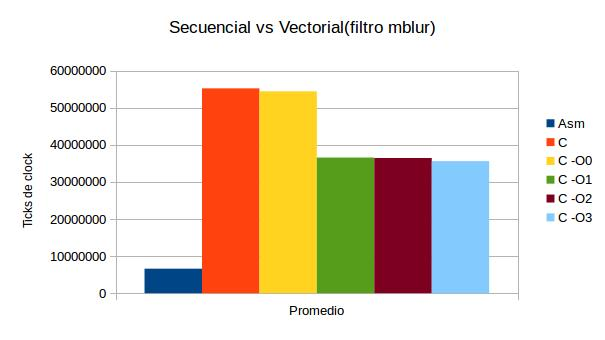
\includegraphics[width=0.7\textwidth]{1exp41a}
\end{figure}
\ \\
\ \\
\begin{figure}[h]
  \centering
    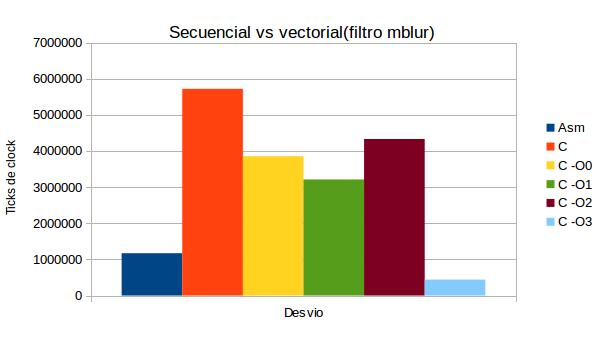
\includegraphics[width=0.7\textwidth]{1exp41b}
\end{figure}
\ \\
Ejecuciones con procesos de fondo:
\ \\
\begin{center}
  \begin{tabular}{| c | c | c | c | c | c |}
    \hline
    ASM & C Com\'un &C -O0 & C -O1 & C -O2 & C -O3\\ 
    \hline\hline

7028607 &54165561 & 108283600 &55304774 & 36276538  &70333140\\
\hline
6067921 &51980211 & 137908488 &35431544 & 34912347 & 69450712\\
\hline
17428782  &51927103& 110948366& 53267979 & 34897387 & 69503896\\
\hline
6056054 &51939743 & 106124251& 36090813  &34899538 & 69440427\\
\hline
6055162 &51918722 & 97325536 & 52284248 & 34897226 & 69452395\\
\hline
6171578 &51925591 & 139943107& 35441175 & 34917320 & 69454792\\
\hline
6057270& 51958043 & 97851481 & 45701347 & 68901527 & 69469463\\
\hline
6100773 &51940695 & 86538067 & 35319999 & 68898909 & 69450636\\
\hline
6077780& 51920440 & 86534939 & 52266627 & 34897625 & 69456824\\
\hline
6060194 &51922148 & 86521687 & 35191326 & 34898730 & 69459960\\

  \hline
  \end{tabular}
\end{center}
\ \\
\ \\
\begin{center}
  \begin{tabular}{| c | c | c | c | c | c | c |}
    \hline
      & ASM & C Com\'un& C -O0 & C -O1 & C -O2 & C -O3 \\
      \hline\hline
      Promedio  & 7310412.1& 52159825.7  &105797952.2 &43629983.2 & 41839714.7 & 69547224.5\\
      \hline
      Desv\'io est\'andar & 3567860.188 &705010.590 & 19659036.034  &8909090.312 & 14268569.116  &276678.882\\
      \hline
  \end{tabular}
\end{center}
\ \\
\ \\
\begin{figure}[h]
  \centering
    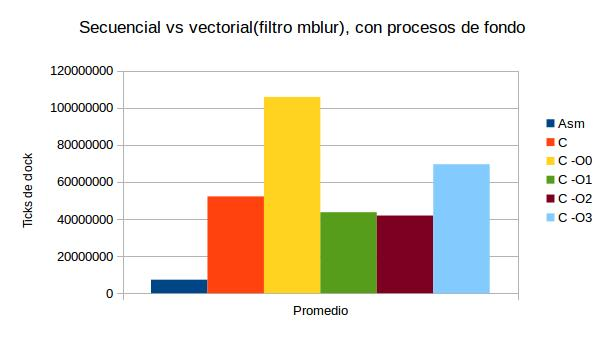
\includegraphics[width=0.7\textwidth]{1exp41c}
\end{figure}
\ \\
\ \\
\begin{figure}[h]
  \centering
    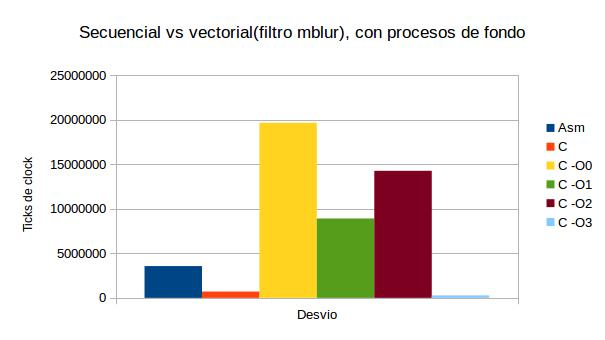
\includegraphics[width=0.7\textwidth]{1exp41d}
\end{figure}
\ \\
Ejecuciones sin los outliers:
\ \\
\begin{center}
  \begin{tabular}{| c | c | c | c | c | c |}
    \hline
    ASM & C Com\'un &C -O0 & C -O1 & C -O2 & C -O3\\ 
    \hline\hline

6475657 &53386860  &53092896  &35605701 & 35305795 & 35457402\\
\hline
6082872 &53402474 & 53290886  &35641333 & 35035853 & 35454715\\
\hline
6083263 &53423766 & 53328311 & 35480725 & 35047948 & 35458166\\
\hline
6191587& 53383341  &53130117  &35603857 & 35042228 & 35451349\\
\hline
6077194 &53402321 & 53055045 & 35478923 & 35009035 & 35463802\\
\hline
6138411 &53403868 & 53331958 & 35570851 & 35029172 & 35453542\\

  \hline
  \end{tabular}
\end{center}
\ \\
\ \\
\begin{center}
  \begin{tabular}{| c | c | c | c | c | c | c |}
    \hline
      & ASM & C Com\'un& C -O0 & C -O1 & C -O2 & C -O3 \\
      \hline\hline
      Promedio  & 6174830.666&  53400438.333 & 53204868.833 & 35563565 & 35078338.5 & 35456496\\
      \hline
      Desv\'io est\'andar & 153933.493 &14424.430  &125985.325 & 68595.290 & 112240.231 & 4367.540\\
      \hline
  \end{tabular}
\end{center}
\ \\
\ \\
\begin{figure}[h]
  \centering
    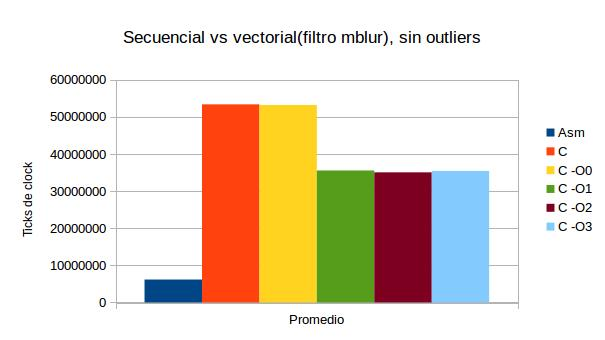
\includegraphics[width=0.7\textwidth]{1exp41e}
\end{figure}
\ \\
\ \\
\begin{figure}[h]
  \centering
    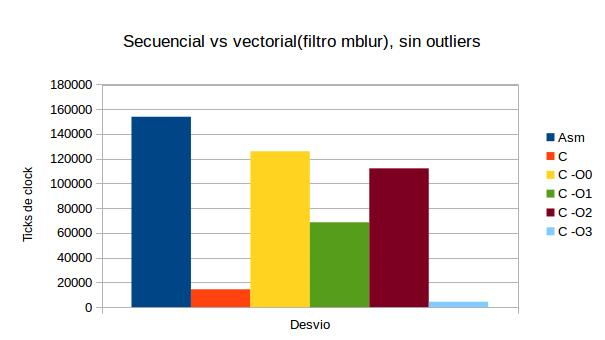
\includegraphics[width=0.7\textwidth]{1exp41f}
\end{figure}
\ \\
\section{Concluci\'on}







\end{document}
